\def\SigmaBlob{plot[smooth cycle,tension=0.7] coordinates {(-3.2,0.1) (-2.6,0.9) (-1.2,1.7) (0.8,1.9) (2.6,1.5) (3.3,0.4) (2.8,-0.9) (1.0,-1.5) (-1.4,-1.4) (-3.0,-0.8)}}

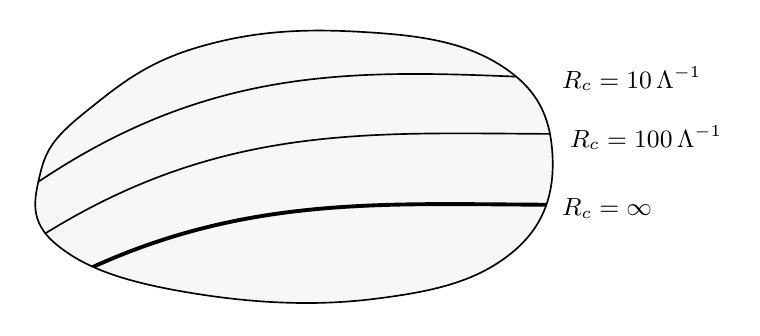
\begin{tikzpicture}[line width=0.6pt]
  \begin{scope}
    \clip \SigmaBlob;
    \fill[gray!6] (-4,-2) rectangle (4,2.2);
    \draw (-3.5,-0.2) .. controls (-1,1.6) and (1,1.4) .. (3.5,1.3);
    \draw (-3.5,-0.9) .. controls (-1,0.8) and (1,0.6) .. (3.5,0.6);
    \draw[line width=1.4pt] (-3.5,-1.6) .. controls (-1,-0.1) and (1,-0.3) .. (3.5,-0.3);
  \end{scope}
  \draw \SigmaBlob;
  \node[right,font=\small] at (3.3,1.3) {$R_c=10\,\Lambda^{-1}$};
  \node[right,font=\small] at (3.4,0.55) {$R_c=100\,\Lambda^{-1}$};
  \node[right,font=\small] at (3.3,-0.35) {$R_c=\infty$};
\end{tikzpicture}
